\chapter{A little bit of theory}
\section{Data structures}
\subsection{¿What is a data structure?}
A simple form to describe this is: a data structure is a container to store data in a specific layout.
This layout allow us to make efficient our data structure in some operations but inefficient in others.

\subsection{¿Why do we need data strucures?}
Depending of different scenarios, data needs to be stored in a specific format, to solve this we need to know the different types of data structures.

\subsection{Basic data structures}
Nowadays there are a lot of types of data structures but here we have a little list of the commonly used data structures.
\begin{itemize}
    \item { Arrays }
    \item { Stacks }
    \item { Queues }
    \item { Linked list }
    \item { Trees }
    \item { Graphs }
    \item { Tries }
    \item { Hash tables }
\end{itemize}

\subsubsection{Arrays}
An array is the simplest used data structure and other data structures can be made using arrays, like stacks and queues. Most of the programming languages index the first element in zero.

We have two types of arrays:
\begin{itemize}
    \item { One-dimensional arrays }
    \item { Multi-dimensional arrays}
\end{itemize}   

\paragraph{Basic operations on arrays}

\begin{enumerate}
    \item { Insert: Inserts an element at given index }
    \item { Get: returns the element at given index }
    \item { Delete: Deletes an element at given index }
    \item { Size: Get the total number of elements in an array }
\end{enumerate}

\paragraph{Commonly asked array interview questions}
\begin{enumerate}
    \item { Find the second minimum element of an array }
    \item { First non-repeating integers in the array }
    \item { Merge two sorted arrays }
    \item { Rearrage positive and negative values in an array }
\end{enumerate}

\subsubsection{Stacks}
This data structure has a lot of applications, for example when we use the undo command.
A stack works like a pile of something for example books. In this example each book are placed in a vertical order. If we have a stack of books we can not get a book placed in the middle, first ypu need to remove all the books on the top to get it.
This behaviour is know as LIFO (Last In First Out) 

\paragraph{Basic operations}
\begin{enumerate}
    \item { Push: inserts an element of the top }
    \item { Pop: returns the top element, after removing from the stack }
    \item { isEmpty: returns true if the stack is is empty }
    \item { Top: returns the top element without removing from the stack }
\end{enumerate}

\paragraph{Commonly asked stack interview questions}
\begin{enumerate}
    \item { Evalue postfix expression using a stack }
    \item { Sort values in a stack }
    \item { Check balanced parentheses in an expression }
\end{enumerate}

\subsubsection{Queues}
Similar to stack, queue is another data structure that stores the element in a sequential manner. The difference is that instead of use LIFO method, queue implements FIFO method (First In First Out)

An example of a queue in real life is a line of people waiting to buy a ticket. If a new person comes, he or she will join the line from the end, not from the start and the person first person (start) will be the first to buy the ticket and then he or she leaves the line.

\paragraph{Basic operations}
\begin{enumerate}
    \item { Enqueue: inserts an element at the end of the queue}
    \item { Dequeue: removes an element from the start of the queue }
    \item { isEmpty: returns true if the queue is empty }
    \item { top: returns the first element of the queue }
\end{enumerate}

\paragraph{Commonly asked queue interview questions}
\begin{enumerate}
    \item { Implement a stack using a queue }
    \item { Reverse first k elements of a queue }
    \item { Generate binary numbers from 1 to n using a queue }
\end{enumerate}

\subsubsection{Linked list}
A linked list is another important data structure that is very similar to an array but differs in memory allocation, internal structure and how basic operations of insertion and deletion are carried out.

A linked list is like a chain of nodes, where each node contains information like data and a ponter to the succeding node in the chain. There's a head pointer, which points to the first element of the linked list, and if the list is empty then it simply points to null or nothing.

Linked lists are used to implement file systems, hash tables, and adjacency lists.

Also exists different types of linked lists:
\begin{itemize}
    \item { Singly linked lists }
    \item { Doubly linked lists }
\end{itemize}

\paragraph{Basic operations}
\begin{enumerate}
    \item { InsertAtEnd: inserts given element at the end of the linked list }
    \item { InsertAtHead: inserts given element at the start/head of the linked list }
    \item { Delete: deletes given element from the linked list }
    \item { DeleteAtHead: deletes first element of the linked list }
    \item { Search: returns the given element from a linked list }
    \item { isEmpty: returns true if the linked list is empty }
\end{enumerate}

\paragraph{Commonly asked linked list interview questions}
\begin{enumerate}
    \item Reverse a linked list
    \item Detect loop in a linked list
    \item Return N-th node from the end in a linked list
    \item Remove duplicates from a linked list
\end{enumerate}

\subsubsection{Graphs}
A graph is a set of nodes that are connected to each other in the form of a network. Nodes are also called vertices. A pair(x, y) is called an edge, which indicates that vertex x is conected to vertex y. An edge may contain weight/cost, showing how much cost is required to traverse from vertex x to y.

Also we have different types of graphs:
\begin{itemize}
    \item { Undirected graphs $ \longrightarrow $ }
    \item { Directed graphs $ \longleftrightarrow $ }
\end{itemize}

We can represent graphs in two forms:
\begin{itemize}
    \item { Adjacency matrix }
    \item { Adjacency list }
\end{itemize}

Finally we have two common graph traversing algorithms:
\begin{itemize}
    \item { Breadth First Search (BFS)}
    \item { Depth First Search (DFS) }
\end{itemize}

\paragraph{Commonly asked graph interview questions}
\begin{enumerate}
    \item { Implement Breath and Depth First Search }
    \item { Check if a graph is tree or not }
    \item { Count number of edges in a graph }
    \item { Find the shortest path between two vertices }
\end{enumerate}

\subsubsection{Trees}
A tree is a special type of graph the difference is that in a tree a cycle cannot exist. This data structure also use vertices (nodes) and edges that connect them.

We have different types of trees:
\begin{itemize}
    \item { N-ary tree }
    \item { Balanced tree }
    \item { Binary tree }
    \item { Binary search tree }
    \item { AVL tree }
    \item { Red-Black tree }
    \item { 2-3 tree }
\end{itemize}

But the most used trees are binary tree and binary search tree.

\paragraph{Commonly asked tree interview questions}
\begin{enumerate}
    \item { Find the heigh of a binary tree }
    \item { Find the k-th maximum value in a binary search tree }
    \item { Find nodes at ''k'' distance from the root }
    \item { Find ancestor of a given node in a binary tree }
\end{enumerate}

\subsubsection{Trie}
Trie is also known as ''prefix trees'', is a data structure very similar to a tree which proves to be quite efficient for solving problems releted to strings. It is commonly used to search words in a dictionary, providing auto suggestions in a search engine, and even for IP routing

\paragraph{Commonly asked trie interview questions}
\begin{enumerate}
    \item { Count total number of words in Trie }
    \item { Print all words stored in Trie }
    \item { Sort elements of an array using trie }
    \item { Form words from a dictionary using trie } 
    \item { Build a T9 dictionary }
\end{enumerate}

\subsubsection{Hash table}
Hashing is a process used to uniquely identify objects and store each object at some pre-calculated unique index called its ''key''. So, the object is stored in the form of a ''key-value'' pair, and the collection of such items called a ''dictionary''. Each object can be searched using that key. There are a lot of data structures based on hashing, but the commonly used data structure is hash table.

Hash tables are commonly implemented using arrays and the performance of hashing data structure depends of three factors:
\begin{itemize}
    \item { Hash function }
    \item { Size of the hash table }
    \item { Collision handling method }
\end{itemize}

\paragraph{Commonly asked hash table interview questions}
\begin{enumerate}
    \item { Find symetric pairs in an array }
    \item { Trace complete path of a journey }
    \item { Find if an array is a subset of another array }
    \item { Check if given arrays are disjoint }
\end{enumerate}

\section{Arrays}
If we are talking about dynamic programming most of the times it is an optimization of a solution that use recursion. As we know most of the times use recursion results in an exponential complexity in time so if we find a way to use dynamic programming we can reduce this complexity.\\

\paragraph{What is the main idea of use Dynamic programming?}
The idea is very simple, if we can store the result of the subproblems, we do not need to re-calculate this subproblem and it reduces the complexity from exponential to a polynomial. 

\subsection{Examples}
We can use the idea of calculate a factorial number, we know that a factorial number it is the multiplication of all the numbers from 1 to n, for example

\begin{itemize}
    \item { Calculate 2! = 1 * 2 = 2}
    \item { Calculate 3! = 1 * 2 * 3 = 6}
    \item { Calculate 5! = 1 * 2 * 3 * 4 * 5  = 120}
\end{itemize}

But we need to consider some things about factorial numbers
\begin{enumerate}
    \item { 0! = 1 }
    \item { Factorial numbers exist in range of $[0, \infty)$ }
\end{enumerate}

If we know this we can notice that we can get a formula to simplify this:
\[
    factorial( n ) = 
    \begin{cases*}
        n * factorial(n - 1) & if $n > 1$ \\
        1 & otherwise
    \end{cases*}
\]

Now we can solve this problem using a recursive program, it is very simple because we just need to programm the formula 
\begin{lstlisting}
    #include<bits/stdc++.h>

    using namespace std;
    typedef long long int lli;
    
    lli factorial( int n ){
        if( n > 1 )
            return n * factorial(n);
        return 1;
    }

    int main(){
        int n;
        cin >> n;
        cout << factorial( n ) << endl;
        return 0;
    }
\end{lstlisting}

If we use the last program we can get the factorial of n, but the complexity of this algorithm is $O(n!)$ so it is awful, but using dynamic programming can we get a better complexity? \\

For me is easier to find a solution using dynamic programming using draws, so I go to make the draw of the recursive calls of the example 5!

\begin{figure}[H]
\begin{center}
    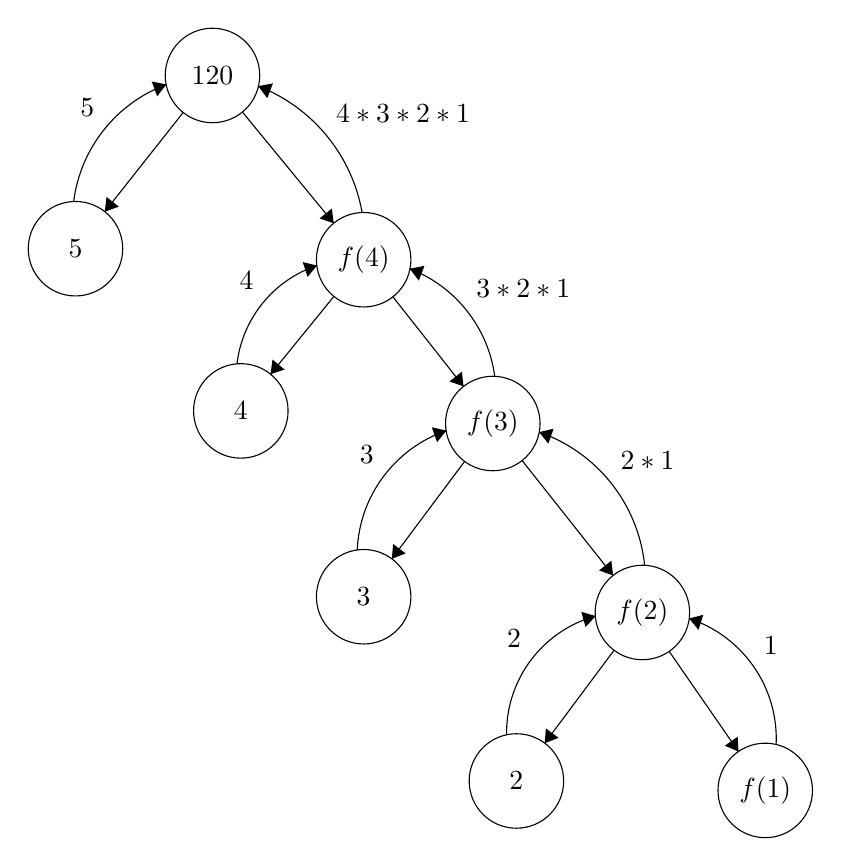
\begin{tikzpicture}[scale=0.2]
    \tikzstyle{every node}+=[inner sep=0pt]
    \draw [black] (30.8,-6.3) circle (3);
    \draw (30.8,-6.3) node {$120$};
    \draw [black] (22.1,-17.3) circle (3);
    \draw (22.1,-17.3) node {$5$};
    \draw [black] (40.4,-18) circle (3);
    \draw (40.4,-18) node {$f(4)$};
    \draw [black] (32.6,-27.6) circle (3);
    \draw (32.6,-27.6) node {$4$};
    \draw [black] (48.6,-28.4) circle (3);
    \draw (48.6,-28.4) node {$f(3)$};
    \draw [black] (40.4,-39.4) circle (3);
    \draw (40.4,-39.4) node {$3$};
    \draw [black] (58.1,-40.4) circle (3);
    \draw (58.1,-40.4) node {$f(2)$};
    \draw [black] (65.9,-51.7) circle (3);
    \draw (65.9,-51.7) node {$f(1)$};
    \draw [black] (50.1,-51.1) circle (3);
    \draw (50.1,-51.1) node {$2$};
    \draw [black] (28.94,-8.65) -- (23.96,-14.95);
    \fill [black] (23.96,-14.95) -- (24.85,-14.63) -- (24.07,-14.01);
    \draw [black] (32.7,-8.62) -- (38.5,-15.68);
    \fill [black] (38.5,-15.68) -- (38.38,-14.75) -- (37.6,-15.38);
    \draw [black] (38.51,-20.33) -- (34.49,-25.27);
    \fill [black] (34.49,-25.27) -- (35.38,-24.97) -- (34.61,-24.34);
    \draw [black] (42.26,-20.36) -- (46.74,-26.04);
    \fill [black] (46.74,-26.04) -- (46.64,-25.11) -- (45.85,-25.73);
    \draw [black] (50.46,-30.75) -- (56.24,-38.05);
    \fill [black] (56.24,-38.05) -- (56.13,-37.11) -- (55.35,-37.73);
    \draw [black] (46.81,-30.81) -- (42.19,-36.99);
    \fill [black] (42.19,-36.99) -- (43.07,-36.65) -- (42.27,-36.05);
    \draw [black] (59.8,-42.87) -- (64.2,-49.23);
    \fill [black] (64.2,-49.23) -- (64.15,-48.29) -- (63.33,-48.86);
    \draw [black] (56.3,-42.8) -- (51.9,-48.7);
    \fill [black] (51.9,-48.7) -- (52.78,-48.36) -- (51.97,-47.76);
    \draw [black] (61.058,-40.782) arc (71.94761:-2.71565:8.032);
    \fill [black] (61.06,-40.78) -- (61.66,-41.5) -- (61.97,-40.55);
    \draw (65.78,-42.5) node [right] {$1$};
    \draw [black] (49.475,-48.185) arc (-179.04361:-254.52464:7.711);
    \fill [black] (55.13,-40.63) -- (54.22,-40.36) -- (54.49,-41.32);
    \draw (50.43,-42.04) node [left] {$2$};
    \draw [black] (51.539,-28.946) arc (70.92086:5.81411:10.037);
    \fill [black] (51.54,-28.95) -- (52.13,-29.68) -- (52.46,-28.73);
    \draw (56.69,-30.78) node [right] {$2*1$};
    \draw [black] (39.992,-36.444) arc (-182.37685:-251.02886:8.395);
    \fill [black] (45.65,-28.85) -- (44.73,-28.64) -- (45.06,-29.59);
    \draw (41.07,-30.38) node [left] {$3$};
    \draw [black] (33.712,-6.98) arc (68.73994:9.99869:10.591);
    \fill [black] (33.71,-6.98) -- (34.28,-7.74) -- (34.64,-6.8);
    \draw (38.62,-8.7) node [right] {$4*3*2*1$};
    \draw [black] (21.983,-14.316) arc (-187.14018:-249.5414:9.158);
    \fill [black] (27.87,-6.87) -- (26.94,-6.68) -- (27.29,-7.62);
    \draw (23.32,-8.35) node [left] {$5$};
    \draw [black] (43.329,-18.572) arc (68.89286:7.61598:8.553);
    \fill [black] (43.33,-18.57) -- (43.9,-19.33) -- (44.26,-18.39);
    \draw (47.53,-19.84) node [right] {$3*2*1$};
    \draw [black] (32.353,-24.63) arc (-186.66238:-251.52534:7.525);
    \fill [black] (37.44,-18.37) -- (36.53,-18.15) -- (36.84,-19.09);
    \draw (33.43,-19.33) node [left] {$4$};
    \end{tikzpicture}
\end{center}
\end{figure}

As we can see we the small problem contains information of the base case has information of the next case and this case has information for the next case and so on, so we do not need to call. Maybe if you need to calculate just once a factorial number it is not necessary to store the information about a factorial number but imagine that you are doing a program that needs a lot of factorial numbers, if we use the recursive algorithm without dynamic programming we need to do for each query $O(n!)$ operations, and that is a lot. So we can store this information and make each query a lot of times and if we already calculated a factorial number we just need to return the information and it is $O(1)$

\begin{lstlisting}
    #include <bits/stdc++.h>

    using namespace std;
    typedef long long int lli;

    vector< lli > factorial_number( 1000 + 1, -1 )
    lli factorial( int n ){

        if( factorial_number[ n ] != -1)
            return factorial_number[ n ];

        if( n > 1 )
            return ( factorial_number[ n ] = (n * factorial( n - 1 ) );

        return factorial_number[ n ] = 1;
    }

    int main(){
        int t, n;
        cin >> t;
        while( t-- ){
            cin >> n;
            cout << n << "! = " << factorial( n ) << endl;
        }
        return 0;  
    }
\end{lstlisting}

As you can see we have a little bit of code but we make more efficient get a factorial number, from $O(n!)$ complexity to $O(1)$ in the case of we already calculated the number, but we are using more memory in this case $O(n)$ in other words we are using a container which size is the biggest factorial that we already calculated.\\\\

Other example is calculate Fibonacci numbers, but first of all we need to know what is a factorial number. A factorial number is defined using the next function.

\[
    fibonacci(n) = 
    \begin{cases*}
        0 & if $n \leq 0$ \\    
        n * ( n - 1 ) + ( n - 2 ) & otherwise 
    \end{cases*}    
\]

As the las example we first of all can sole this problem using a recursive algorithm, we just need to program the previous definition of a fibonacci number.

\begin{lstlisting}
    #include<bits/stdc++.h>

    using namespace std;
    typedef long long int lli;

    lli fibonacci( int n ){
        if( n <= 0 )
            return 0;
        return ( n + fibonacci( n - 1 ) + fibonacci( n - 2 ) );
    }

    int main(){
        int n;
        return 0;
    }
\end{lstlisting}



\section{Stacks}
If we are talking about dynamic programming most of the times it is an optimization of a solution that use recursion. As we know most of the times use recursion results in an exponential complexity in time so if we find a way to use dynamic programming we can reduce this complexity.\\

\paragraph{What is the main idea of use Dynamic programming?}
The idea is very simple, if we can store the result of the subproblems, we do not need to re-calculate this subproblem and it reduces the complexity from exponential to a polynomial. 

\subsection{Examples}
We can use the idea of calculate a factorial number, we know that a factorial number it is the multiplication of all the numbers from 1 to n, for example

\begin{itemize}
    \item { Calculate 2! = 1 * 2 = 2}
    \item { Calculate 3! = 1 * 2 * 3 = 6}
    \item { Calculate 5! = 1 * 2 * 3 * 4 * 5  = 120}
\end{itemize}

But we need to consider some things about factorial numbers
\begin{enumerate}
    \item { 0! = 1 }
    \item { Factorial numbers exist in range of $[0, \infty)$ }
\end{enumerate}

If we know this we can notice that we can get a formula to simplify this:
\[
    factorial( n ) = 
    \begin{cases*}
        n * factorial(n - 1) & if $n > 1$ \\
        1 & otherwise
    \end{cases*}
\]

Now we can solve this problem using a recursive program, it is very simple because we just need to programm the formula 
\begin{lstlisting}
    #include<bits/stdc++.h>

    using namespace std;
    typedef long long int lli;
    
    lli factorial( int n ){
        if( n > 1 )
            return n * factorial(n);
        return 1;
    }

    int main(){
        int n;
        cin >> n;
        cout << factorial( n ) << endl;
        return 0;
    }
\end{lstlisting}

If we use the last program we can get the factorial of n, but the complexity of this algorithm is $O(n!)$ so it is awful, but using dynamic programming can we get a better complexity? \\

For me is easier to find a solution using dynamic programming using draws, so I go to make the draw of the recursive calls of the example 5!

\begin{figure}[H]
\begin{center}
    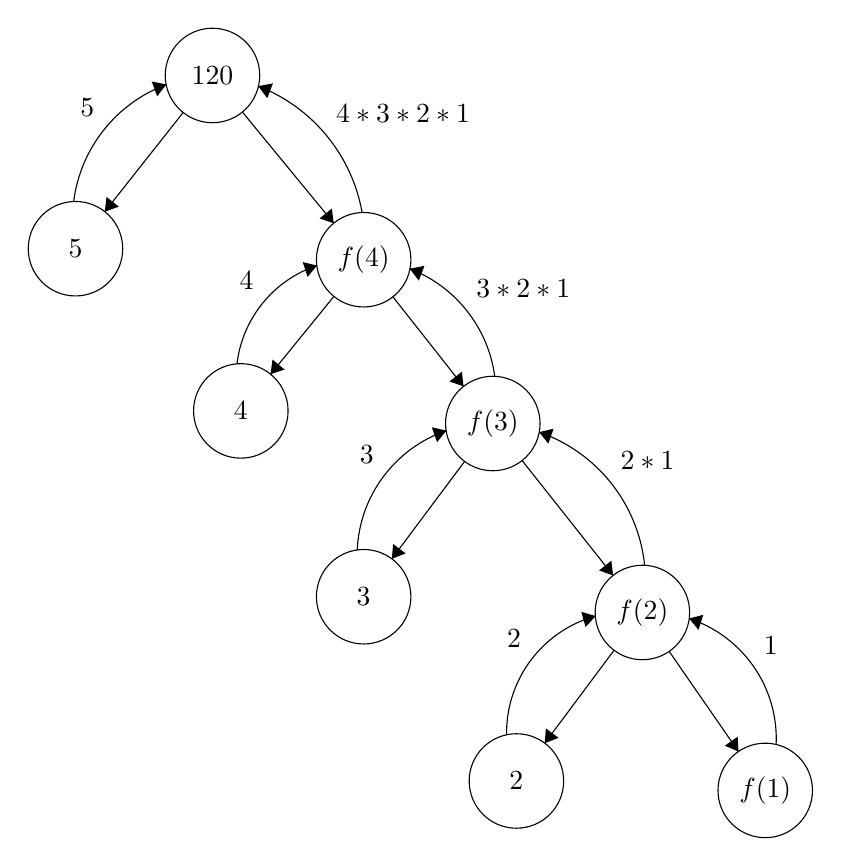
\begin{tikzpicture}[scale=0.2]
    \tikzstyle{every node}+=[inner sep=0pt]
    \draw [black] (30.8,-6.3) circle (3);
    \draw (30.8,-6.3) node {$120$};
    \draw [black] (22.1,-17.3) circle (3);
    \draw (22.1,-17.3) node {$5$};
    \draw [black] (40.4,-18) circle (3);
    \draw (40.4,-18) node {$f(4)$};
    \draw [black] (32.6,-27.6) circle (3);
    \draw (32.6,-27.6) node {$4$};
    \draw [black] (48.6,-28.4) circle (3);
    \draw (48.6,-28.4) node {$f(3)$};
    \draw [black] (40.4,-39.4) circle (3);
    \draw (40.4,-39.4) node {$3$};
    \draw [black] (58.1,-40.4) circle (3);
    \draw (58.1,-40.4) node {$f(2)$};
    \draw [black] (65.9,-51.7) circle (3);
    \draw (65.9,-51.7) node {$f(1)$};
    \draw [black] (50.1,-51.1) circle (3);
    \draw (50.1,-51.1) node {$2$};
    \draw [black] (28.94,-8.65) -- (23.96,-14.95);
    \fill [black] (23.96,-14.95) -- (24.85,-14.63) -- (24.07,-14.01);
    \draw [black] (32.7,-8.62) -- (38.5,-15.68);
    \fill [black] (38.5,-15.68) -- (38.38,-14.75) -- (37.6,-15.38);
    \draw [black] (38.51,-20.33) -- (34.49,-25.27);
    \fill [black] (34.49,-25.27) -- (35.38,-24.97) -- (34.61,-24.34);
    \draw [black] (42.26,-20.36) -- (46.74,-26.04);
    \fill [black] (46.74,-26.04) -- (46.64,-25.11) -- (45.85,-25.73);
    \draw [black] (50.46,-30.75) -- (56.24,-38.05);
    \fill [black] (56.24,-38.05) -- (56.13,-37.11) -- (55.35,-37.73);
    \draw [black] (46.81,-30.81) -- (42.19,-36.99);
    \fill [black] (42.19,-36.99) -- (43.07,-36.65) -- (42.27,-36.05);
    \draw [black] (59.8,-42.87) -- (64.2,-49.23);
    \fill [black] (64.2,-49.23) -- (64.15,-48.29) -- (63.33,-48.86);
    \draw [black] (56.3,-42.8) -- (51.9,-48.7);
    \fill [black] (51.9,-48.7) -- (52.78,-48.36) -- (51.97,-47.76);
    \draw [black] (61.058,-40.782) arc (71.94761:-2.71565:8.032);
    \fill [black] (61.06,-40.78) -- (61.66,-41.5) -- (61.97,-40.55);
    \draw (65.78,-42.5) node [right] {$1$};
    \draw [black] (49.475,-48.185) arc (-179.04361:-254.52464:7.711);
    \fill [black] (55.13,-40.63) -- (54.22,-40.36) -- (54.49,-41.32);
    \draw (50.43,-42.04) node [left] {$2$};
    \draw [black] (51.539,-28.946) arc (70.92086:5.81411:10.037);
    \fill [black] (51.54,-28.95) -- (52.13,-29.68) -- (52.46,-28.73);
    \draw (56.69,-30.78) node [right] {$2*1$};
    \draw [black] (39.992,-36.444) arc (-182.37685:-251.02886:8.395);
    \fill [black] (45.65,-28.85) -- (44.73,-28.64) -- (45.06,-29.59);
    \draw (41.07,-30.38) node [left] {$3$};
    \draw [black] (33.712,-6.98) arc (68.73994:9.99869:10.591);
    \fill [black] (33.71,-6.98) -- (34.28,-7.74) -- (34.64,-6.8);
    \draw (38.62,-8.7) node [right] {$4*3*2*1$};
    \draw [black] (21.983,-14.316) arc (-187.14018:-249.5414:9.158);
    \fill [black] (27.87,-6.87) -- (26.94,-6.68) -- (27.29,-7.62);
    \draw (23.32,-8.35) node [left] {$5$};
    \draw [black] (43.329,-18.572) arc (68.89286:7.61598:8.553);
    \fill [black] (43.33,-18.57) -- (43.9,-19.33) -- (44.26,-18.39);
    \draw (47.53,-19.84) node [right] {$3*2*1$};
    \draw [black] (32.353,-24.63) arc (-186.66238:-251.52534:7.525);
    \fill [black] (37.44,-18.37) -- (36.53,-18.15) -- (36.84,-19.09);
    \draw (33.43,-19.33) node [left] {$4$};
    \end{tikzpicture}
\end{center}
\end{figure}

As we can see we the small problem contains information of the base case has information of the next case and this case has information for the next case and so on, so we do not need to call. Maybe if you need to calculate just once a factorial number it is not necessary to store the information about a factorial number but imagine that you are doing a program that needs a lot of factorial numbers, if we use the recursive algorithm without dynamic programming we need to do for each query $O(n!)$ operations, and that is a lot. So we can store this information and make each query a lot of times and if we already calculated a factorial number we just need to return the information and it is $O(1)$

\begin{lstlisting}
    #include <bits/stdc++.h>

    using namespace std;
    typedef long long int lli;

    vector< lli > factorial_number( 1000 + 1, -1 )
    lli factorial( int n ){

        if( factorial_number[ n ] != -1)
            return factorial_number[ n ];

        if( n > 1 )
            return ( factorial_number[ n ] = (n * factorial( n - 1 ) );

        return factorial_number[ n ] = 1;
    }

    int main(){
        int t, n;
        cin >> t;
        while( t-- ){
            cin >> n;
            cout << n << "! = " << factorial( n ) << endl;
        }
        return 0;  
    }
\end{lstlisting}

As you can see we have a little bit of code but we make more efficient get a factorial number, from $O(n!)$ complexity to $O(1)$ in the case of we already calculated the number, but we are using more memory in this case $O(n)$ in other words we are using a container which size is the biggest factorial that we already calculated.\\\\

Other example is calculate Fibonacci numbers, but first of all we need to know what is a factorial number. A factorial number is defined using the next function.

\[
    fibonacci(n) = 
    \begin{cases*}
        0 & if $n \leq 0$ \\    
        n * ( n - 1 ) + ( n - 2 ) & otherwise 
    \end{cases*}    
\]

As the las example we first of all can sole this problem using a recursive algorithm, we just need to program the previous definition of a fibonacci number.

\begin{lstlisting}
    #include<bits/stdc++.h>

    using namespace std;
    typedef long long int lli;

    lli fibonacci( int n ){
        if( n <= 0 )
            return 0;
        return ( n + fibonacci( n - 1 ) + fibonacci( n - 2 ) );
    }

    int main(){
        int n;
        return 0;
    }
\end{lstlisting}



\section{Queues}
If we are talking about dynamic programming most of the times it is an optimization of a solution that use recursion. As we know most of the times use recursion results in an exponential complexity in time so if we find a way to use dynamic programming we can reduce this complexity.\\

\paragraph{What is the main idea of use Dynamic programming?}
The idea is very simple, if we can store the result of the subproblems, we do not need to re-calculate this subproblem and it reduces the complexity from exponential to a polynomial. 

\subsection{Examples}
We can use the idea of calculate a factorial number, we know that a factorial number it is the multiplication of all the numbers from 1 to n, for example

\begin{itemize}
    \item { Calculate 2! = 1 * 2 = 2}
    \item { Calculate 3! = 1 * 2 * 3 = 6}
    \item { Calculate 5! = 1 * 2 * 3 * 4 * 5  = 120}
\end{itemize}

But we need to consider some things about factorial numbers
\begin{enumerate}
    \item { 0! = 1 }
    \item { Factorial numbers exist in range of $[0, \infty)$ }
\end{enumerate}

If we know this we can notice that we can get a formula to simplify this:
\[
    factorial( n ) = 
    \begin{cases*}
        n * factorial(n - 1) & if $n > 1$ \\
        1 & otherwise
    \end{cases*}
\]

Now we can solve this problem using a recursive program, it is very simple because we just need to programm the formula 
\begin{lstlisting}
    #include<bits/stdc++.h>

    using namespace std;
    typedef long long int lli;
    
    lli factorial( int n ){
        if( n > 1 )
            return n * factorial(n);
        return 1;
    }

    int main(){
        int n;
        cin >> n;
        cout << factorial( n ) << endl;
        return 0;
    }
\end{lstlisting}

If we use the last program we can get the factorial of n, but the complexity of this algorithm is $O(n!)$ so it is awful, but using dynamic programming can we get a better complexity? \\

For me is easier to find a solution using dynamic programming using draws, so I go to make the draw of the recursive calls of the example 5!

\begin{figure}[H]
\begin{center}
    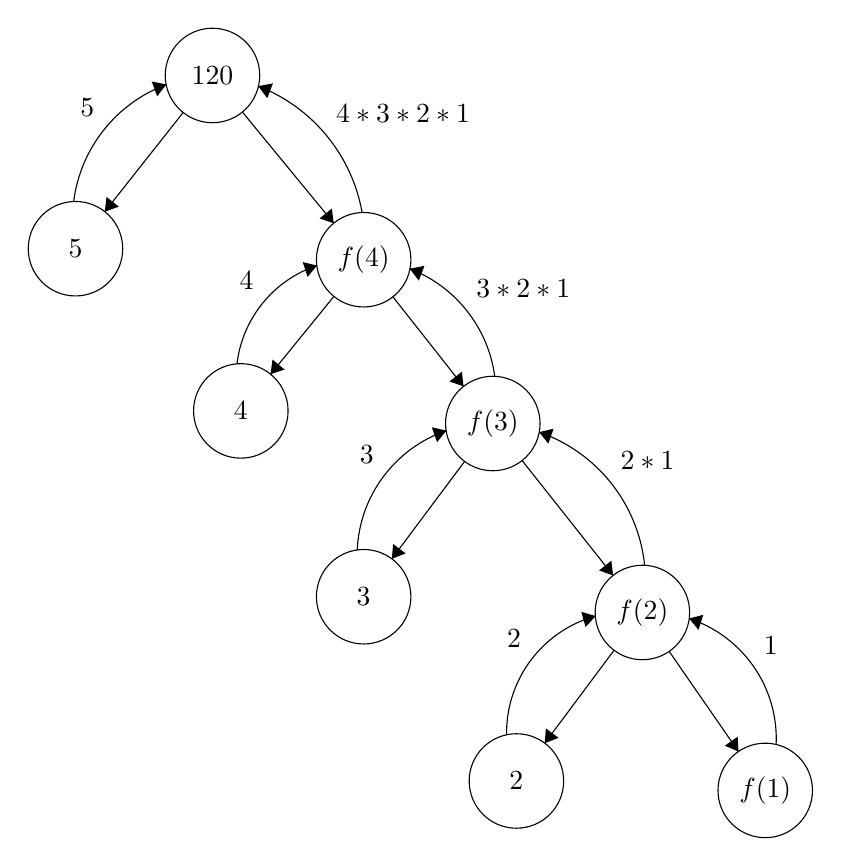
\begin{tikzpicture}[scale=0.2]
    \tikzstyle{every node}+=[inner sep=0pt]
    \draw [black] (30.8,-6.3) circle (3);
    \draw (30.8,-6.3) node {$120$};
    \draw [black] (22.1,-17.3) circle (3);
    \draw (22.1,-17.3) node {$5$};
    \draw [black] (40.4,-18) circle (3);
    \draw (40.4,-18) node {$f(4)$};
    \draw [black] (32.6,-27.6) circle (3);
    \draw (32.6,-27.6) node {$4$};
    \draw [black] (48.6,-28.4) circle (3);
    \draw (48.6,-28.4) node {$f(3)$};
    \draw [black] (40.4,-39.4) circle (3);
    \draw (40.4,-39.4) node {$3$};
    \draw [black] (58.1,-40.4) circle (3);
    \draw (58.1,-40.4) node {$f(2)$};
    \draw [black] (65.9,-51.7) circle (3);
    \draw (65.9,-51.7) node {$f(1)$};
    \draw [black] (50.1,-51.1) circle (3);
    \draw (50.1,-51.1) node {$2$};
    \draw [black] (28.94,-8.65) -- (23.96,-14.95);
    \fill [black] (23.96,-14.95) -- (24.85,-14.63) -- (24.07,-14.01);
    \draw [black] (32.7,-8.62) -- (38.5,-15.68);
    \fill [black] (38.5,-15.68) -- (38.38,-14.75) -- (37.6,-15.38);
    \draw [black] (38.51,-20.33) -- (34.49,-25.27);
    \fill [black] (34.49,-25.27) -- (35.38,-24.97) -- (34.61,-24.34);
    \draw [black] (42.26,-20.36) -- (46.74,-26.04);
    \fill [black] (46.74,-26.04) -- (46.64,-25.11) -- (45.85,-25.73);
    \draw [black] (50.46,-30.75) -- (56.24,-38.05);
    \fill [black] (56.24,-38.05) -- (56.13,-37.11) -- (55.35,-37.73);
    \draw [black] (46.81,-30.81) -- (42.19,-36.99);
    \fill [black] (42.19,-36.99) -- (43.07,-36.65) -- (42.27,-36.05);
    \draw [black] (59.8,-42.87) -- (64.2,-49.23);
    \fill [black] (64.2,-49.23) -- (64.15,-48.29) -- (63.33,-48.86);
    \draw [black] (56.3,-42.8) -- (51.9,-48.7);
    \fill [black] (51.9,-48.7) -- (52.78,-48.36) -- (51.97,-47.76);
    \draw [black] (61.058,-40.782) arc (71.94761:-2.71565:8.032);
    \fill [black] (61.06,-40.78) -- (61.66,-41.5) -- (61.97,-40.55);
    \draw (65.78,-42.5) node [right] {$1$};
    \draw [black] (49.475,-48.185) arc (-179.04361:-254.52464:7.711);
    \fill [black] (55.13,-40.63) -- (54.22,-40.36) -- (54.49,-41.32);
    \draw (50.43,-42.04) node [left] {$2$};
    \draw [black] (51.539,-28.946) arc (70.92086:5.81411:10.037);
    \fill [black] (51.54,-28.95) -- (52.13,-29.68) -- (52.46,-28.73);
    \draw (56.69,-30.78) node [right] {$2*1$};
    \draw [black] (39.992,-36.444) arc (-182.37685:-251.02886:8.395);
    \fill [black] (45.65,-28.85) -- (44.73,-28.64) -- (45.06,-29.59);
    \draw (41.07,-30.38) node [left] {$3$};
    \draw [black] (33.712,-6.98) arc (68.73994:9.99869:10.591);
    \fill [black] (33.71,-6.98) -- (34.28,-7.74) -- (34.64,-6.8);
    \draw (38.62,-8.7) node [right] {$4*3*2*1$};
    \draw [black] (21.983,-14.316) arc (-187.14018:-249.5414:9.158);
    \fill [black] (27.87,-6.87) -- (26.94,-6.68) -- (27.29,-7.62);
    \draw (23.32,-8.35) node [left] {$5$};
    \draw [black] (43.329,-18.572) arc (68.89286:7.61598:8.553);
    \fill [black] (43.33,-18.57) -- (43.9,-19.33) -- (44.26,-18.39);
    \draw (47.53,-19.84) node [right] {$3*2*1$};
    \draw [black] (32.353,-24.63) arc (-186.66238:-251.52534:7.525);
    \fill [black] (37.44,-18.37) -- (36.53,-18.15) -- (36.84,-19.09);
    \draw (33.43,-19.33) node [left] {$4$};
    \end{tikzpicture}
\end{center}
\end{figure}

As we can see we the small problem contains information of the base case has information of the next case and this case has information for the next case and so on, so we do not need to call. Maybe if you need to calculate just once a factorial number it is not necessary to store the information about a factorial number but imagine that you are doing a program that needs a lot of factorial numbers, if we use the recursive algorithm without dynamic programming we need to do for each query $O(n!)$ operations, and that is a lot. So we can store this information and make each query a lot of times and if we already calculated a factorial number we just need to return the information and it is $O(1)$

\begin{lstlisting}
    #include <bits/stdc++.h>

    using namespace std;
    typedef long long int lli;

    vector< lli > factorial_number( 1000 + 1, -1 )
    lli factorial( int n ){

        if( factorial_number[ n ] != -1)
            return factorial_number[ n ];

        if( n > 1 )
            return ( factorial_number[ n ] = (n * factorial( n - 1 ) );

        return factorial_number[ n ] = 1;
    }

    int main(){
        int t, n;
        cin >> t;
        while( t-- ){
            cin >> n;
            cout << n << "! = " << factorial( n ) << endl;
        }
        return 0;  
    }
\end{lstlisting}

As you can see we have a little bit of code but we make more efficient get a factorial number, from $O(n!)$ complexity to $O(1)$ in the case of we already calculated the number, but we are using more memory in this case $O(n)$ in other words we are using a container which size is the biggest factorial that we already calculated.\\\\

Other example is calculate Fibonacci numbers, but first of all we need to know what is a factorial number. A factorial number is defined using the next function.

\[
    fibonacci(n) = 
    \begin{cases*}
        0 & if $n \leq 0$ \\    
        n * ( n - 1 ) + ( n - 2 ) & otherwise 
    \end{cases*}    
\]

As the las example we first of all can sole this problem using a recursive algorithm, we just need to program the previous definition of a fibonacci number.

\begin{lstlisting}
    #include<bits/stdc++.h>

    using namespace std;
    typedef long long int lli;

    lli fibonacci( int n ){
        if( n <= 0 )
            return 0;
        return ( n + fibonacci( n - 1 ) + fibonacci( n - 2 ) );
    }

    int main(){
        int n;
        return 0;
    }
\end{lstlisting}



\section{Singly linked lists}
If we are talking about dynamic programming most of the times it is an optimization of a solution that use recursion. As we know most of the times use recursion results in an exponential complexity in time so if we find a way to use dynamic programming we can reduce this complexity.\\

\paragraph{What is the main idea of use Dynamic programming?}
The idea is very simple, if we can store the result of the subproblems, we do not need to re-calculate this subproblem and it reduces the complexity from exponential to a polynomial. 

\subsection{Examples}
We can use the idea of calculate a factorial number, we know that a factorial number it is the multiplication of all the numbers from 1 to n, for example

\begin{itemize}
    \item { Calculate 2! = 1 * 2 = 2}
    \item { Calculate 3! = 1 * 2 * 3 = 6}
    \item { Calculate 5! = 1 * 2 * 3 * 4 * 5  = 120}
\end{itemize}

But we need to consider some things about factorial numbers
\begin{enumerate}
    \item { 0! = 1 }
    \item { Factorial numbers exist in range of $[0, \infty)$ }
\end{enumerate}

If we know this we can notice that we can get a formula to simplify this:
\[
    factorial( n ) = 
    \begin{cases*}
        n * factorial(n - 1) & if $n > 1$ \\
        1 & otherwise
    \end{cases*}
\]

Now we can solve this problem using a recursive program, it is very simple because we just need to programm the formula 
\begin{lstlisting}
    #include<bits/stdc++.h>

    using namespace std;
    typedef long long int lli;
    
    lli factorial( int n ){
        if( n > 1 )
            return n * factorial(n);
        return 1;
    }

    int main(){
        int n;
        cin >> n;
        cout << factorial( n ) << endl;
        return 0;
    }
\end{lstlisting}

If we use the last program we can get the factorial of n, but the complexity of this algorithm is $O(n!)$ so it is awful, but using dynamic programming can we get a better complexity? \\

For me is easier to find a solution using dynamic programming using draws, so I go to make the draw of the recursive calls of the example 5!

\begin{figure}[H]
\begin{center}
    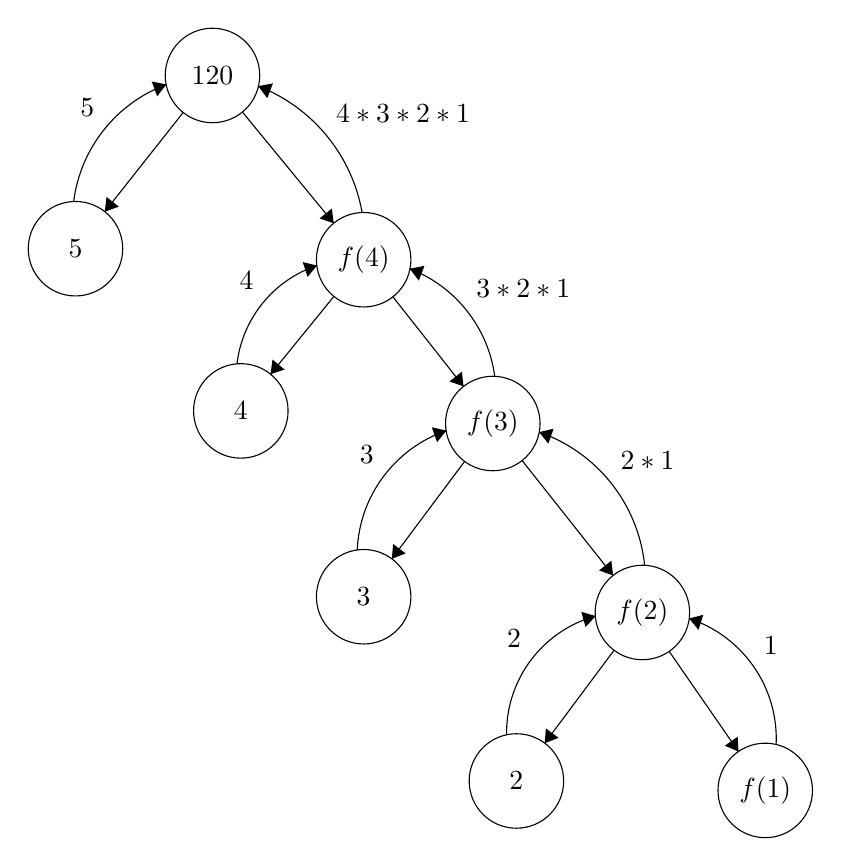
\begin{tikzpicture}[scale=0.2]
    \tikzstyle{every node}+=[inner sep=0pt]
    \draw [black] (30.8,-6.3) circle (3);
    \draw (30.8,-6.3) node {$120$};
    \draw [black] (22.1,-17.3) circle (3);
    \draw (22.1,-17.3) node {$5$};
    \draw [black] (40.4,-18) circle (3);
    \draw (40.4,-18) node {$f(4)$};
    \draw [black] (32.6,-27.6) circle (3);
    \draw (32.6,-27.6) node {$4$};
    \draw [black] (48.6,-28.4) circle (3);
    \draw (48.6,-28.4) node {$f(3)$};
    \draw [black] (40.4,-39.4) circle (3);
    \draw (40.4,-39.4) node {$3$};
    \draw [black] (58.1,-40.4) circle (3);
    \draw (58.1,-40.4) node {$f(2)$};
    \draw [black] (65.9,-51.7) circle (3);
    \draw (65.9,-51.7) node {$f(1)$};
    \draw [black] (50.1,-51.1) circle (3);
    \draw (50.1,-51.1) node {$2$};
    \draw [black] (28.94,-8.65) -- (23.96,-14.95);
    \fill [black] (23.96,-14.95) -- (24.85,-14.63) -- (24.07,-14.01);
    \draw [black] (32.7,-8.62) -- (38.5,-15.68);
    \fill [black] (38.5,-15.68) -- (38.38,-14.75) -- (37.6,-15.38);
    \draw [black] (38.51,-20.33) -- (34.49,-25.27);
    \fill [black] (34.49,-25.27) -- (35.38,-24.97) -- (34.61,-24.34);
    \draw [black] (42.26,-20.36) -- (46.74,-26.04);
    \fill [black] (46.74,-26.04) -- (46.64,-25.11) -- (45.85,-25.73);
    \draw [black] (50.46,-30.75) -- (56.24,-38.05);
    \fill [black] (56.24,-38.05) -- (56.13,-37.11) -- (55.35,-37.73);
    \draw [black] (46.81,-30.81) -- (42.19,-36.99);
    \fill [black] (42.19,-36.99) -- (43.07,-36.65) -- (42.27,-36.05);
    \draw [black] (59.8,-42.87) -- (64.2,-49.23);
    \fill [black] (64.2,-49.23) -- (64.15,-48.29) -- (63.33,-48.86);
    \draw [black] (56.3,-42.8) -- (51.9,-48.7);
    \fill [black] (51.9,-48.7) -- (52.78,-48.36) -- (51.97,-47.76);
    \draw [black] (61.058,-40.782) arc (71.94761:-2.71565:8.032);
    \fill [black] (61.06,-40.78) -- (61.66,-41.5) -- (61.97,-40.55);
    \draw (65.78,-42.5) node [right] {$1$};
    \draw [black] (49.475,-48.185) arc (-179.04361:-254.52464:7.711);
    \fill [black] (55.13,-40.63) -- (54.22,-40.36) -- (54.49,-41.32);
    \draw (50.43,-42.04) node [left] {$2$};
    \draw [black] (51.539,-28.946) arc (70.92086:5.81411:10.037);
    \fill [black] (51.54,-28.95) -- (52.13,-29.68) -- (52.46,-28.73);
    \draw (56.69,-30.78) node [right] {$2*1$};
    \draw [black] (39.992,-36.444) arc (-182.37685:-251.02886:8.395);
    \fill [black] (45.65,-28.85) -- (44.73,-28.64) -- (45.06,-29.59);
    \draw (41.07,-30.38) node [left] {$3$};
    \draw [black] (33.712,-6.98) arc (68.73994:9.99869:10.591);
    \fill [black] (33.71,-6.98) -- (34.28,-7.74) -- (34.64,-6.8);
    \draw (38.62,-8.7) node [right] {$4*3*2*1$};
    \draw [black] (21.983,-14.316) arc (-187.14018:-249.5414:9.158);
    \fill [black] (27.87,-6.87) -- (26.94,-6.68) -- (27.29,-7.62);
    \draw (23.32,-8.35) node [left] {$5$};
    \draw [black] (43.329,-18.572) arc (68.89286:7.61598:8.553);
    \fill [black] (43.33,-18.57) -- (43.9,-19.33) -- (44.26,-18.39);
    \draw (47.53,-19.84) node [right] {$3*2*1$};
    \draw [black] (32.353,-24.63) arc (-186.66238:-251.52534:7.525);
    \fill [black] (37.44,-18.37) -- (36.53,-18.15) -- (36.84,-19.09);
    \draw (33.43,-19.33) node [left] {$4$};
    \end{tikzpicture}
\end{center}
\end{figure}

As we can see we the small problem contains information of the base case has information of the next case and this case has information for the next case and so on, so we do not need to call. Maybe if you need to calculate just once a factorial number it is not necessary to store the information about a factorial number but imagine that you are doing a program that needs a lot of factorial numbers, if we use the recursive algorithm without dynamic programming we need to do for each query $O(n!)$ operations, and that is a lot. So we can store this information and make each query a lot of times and if we already calculated a factorial number we just need to return the information and it is $O(1)$

\begin{lstlisting}
    #include <bits/stdc++.h>

    using namespace std;
    typedef long long int lli;

    vector< lli > factorial_number( 1000 + 1, -1 )
    lli factorial( int n ){

        if( factorial_number[ n ] != -1)
            return factorial_number[ n ];

        if( n > 1 )
            return ( factorial_number[ n ] = (n * factorial( n - 1 ) );

        return factorial_number[ n ] = 1;
    }

    int main(){
        int t, n;
        cin >> t;
        while( t-- ){
            cin >> n;
            cout << n << "! = " << factorial( n ) << endl;
        }
        return 0;  
    }
\end{lstlisting}

As you can see we have a little bit of code but we make more efficient get a factorial number, from $O(n!)$ complexity to $O(1)$ in the case of we already calculated the number, but we are using more memory in this case $O(n)$ in other words we are using a container which size is the biggest factorial that we already calculated.\\\\

Other example is calculate Fibonacci numbers, but first of all we need to know what is a factorial number. A factorial number is defined using the next function.

\[
    fibonacci(n) = 
    \begin{cases*}
        0 & if $n \leq 0$ \\    
        n * ( n - 1 ) + ( n - 2 ) & otherwise 
    \end{cases*}    
\]

As the las example we first of all can sole this problem using a recursive algorithm, we just need to program the previous definition of a fibonacci number.

\begin{lstlisting}
    #include<bits/stdc++.h>

    using namespace std;
    typedef long long int lli;

    lli fibonacci( int n ){
        if( n <= 0 )
            return 0;
        return ( n + fibonacci( n - 1 ) + fibonacci( n - 2 ) );
    }

    int main(){
        int n;
        return 0;
    }
\end{lstlisting}




\section{Doubly linked lists}


\section{Graphs}

\section{Trees}

\section{Tries}